\subsection{Rancangan Behavioural}
\label{subsec:arsitektur-behavioural}

Berdasarkan \textit{use case} diagram yang telah dibuat, terdapat 13 \textit{use case} yang memiliki alur yang berbeda. Untuk menjelaskan interaksi aktor, sistem, serta objek secara terperinci digunakan diagram \textit{sequence}. Terdapat 13 \textit{sequence} pada sistem ini, diagram ini sudah termasuk interaksi antara sistem \textit{dashboard} dan service.

\subsubsection{Alur Mendaftarkan \textit{company}}

Pada \textit{use case} ini, admin yang berperan untuk mendaftarakan \textit{company} baru yang ingin mendaftarkan ke dalam sistem. Admin dapat melakukan request melalui HTTP Client ke server. Server melakukan validasi data dan apabila telah pass, server memasukan informasi ke \textit{database}. Akhirnya, server memberikan response berupa objek dari \textit{company} yang dapat digunakan. Ilustrasi \textit{sequence diagram} dapat dilihat pada gambar \ref{fig:usecase-01}.

\begin{figure}[ht]
  \centering
  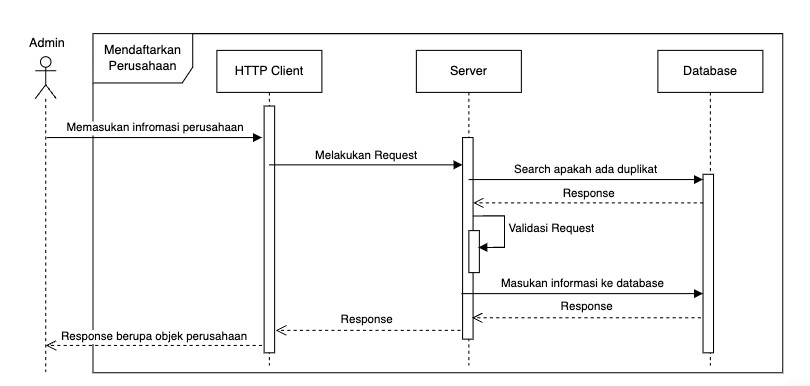
\includegraphics[width=0.7\textwidth]{resources/chapter-3/usecase/uc-01.jpg}
  \caption{\textit{Use Case} Mendaftarkan \textit{Company}}
  \label{fig:usecase-01}
\end{figure}

\subsubsection{Alur Mendaftarkan \textit{User}}

Pada \textit{use case} ini, admin yang berperan untuk mendaftarakan \textit{user} baru yang ingin mendaftarkan ke dalam sistem. Admin dapat melakukan request melalui HTTP Client ke server. Server melakukan validasi data dan apabila telah pass, server memasukan informasi ke \textit{database}. Akhirnya, server memberikan response berupa objek \textit{user} yang dapat digunakan untuk login oleh \textit{user}. Ilustrasi \textit{sequence diagram} dapat dilihat pada gambar \ref{fig:usecase-02}.

\begin{figure}[ht]
  \centering
  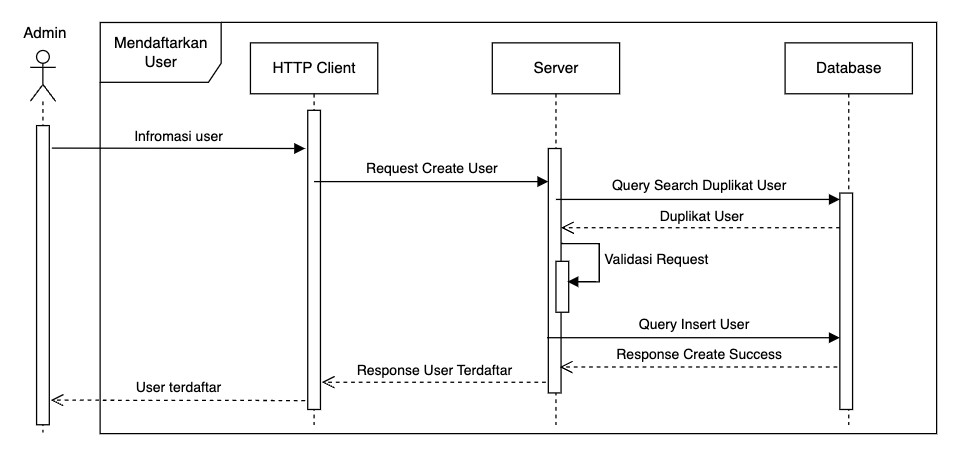
\includegraphics[width=0.8\textwidth]{resources/chapter-3/usecase/uc-02.jpg}
  \caption{\textit{Use Case} Mendaftarkan \textit{User}}
  \label{fig:usecase-02}
\end{figure}

\pagebreak

\subsubsection{Alur Manajemen \textit{company}}

Pada \textit{use case} ini, admin yang berperan untuk melakukan manajemen \textit{company}. Admin dapat menghapus ataupun mengupdate detail \textit{company}. Server melakukan validasi data, setelah melewati seluruh validasi, server melakukan update informasi yang diberikan ke \textit{database}. Server memberikan repsonse berupa hasil update. Ilustrasi \textit{sequence diagram} dapat dilihat pada gambar \ref{fig:usecase-03}.

\begin{figure}[ht]
  \centering
  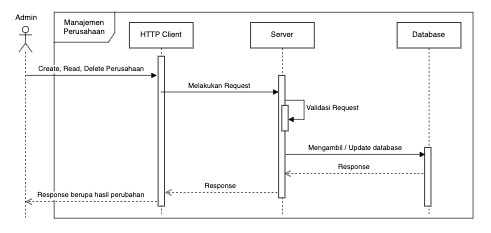
\includegraphics[width=0.8\textwidth]{resources/chapter-3/usecase/uc-03.jpg}
  \caption{\textit{Use Case} Manajemen \textit{Company}}
  \label{fig:usecase-03}
\end{figure}

\subsubsection{Alur Manajemen \textit{User}}

Pada \textit{use case} ini, admin yang berperan untuk melakukan manajemen \textit{user}. Admin dapat menghapus ataupun mengupdate detail \textit{user}. Server melakukan validasi data dan apabila telah pass, server melakukan update informasi yang diberikan ke \textit{database}. Setelah itu server memberikan repsonse berupa hasil update yang telah dilakukan. Ilustrasi \textit{sequence diagram} dapat dilihat pada gambar \ref{fig:usecase-04}.

\begin{figure}[ht]
  \centering
  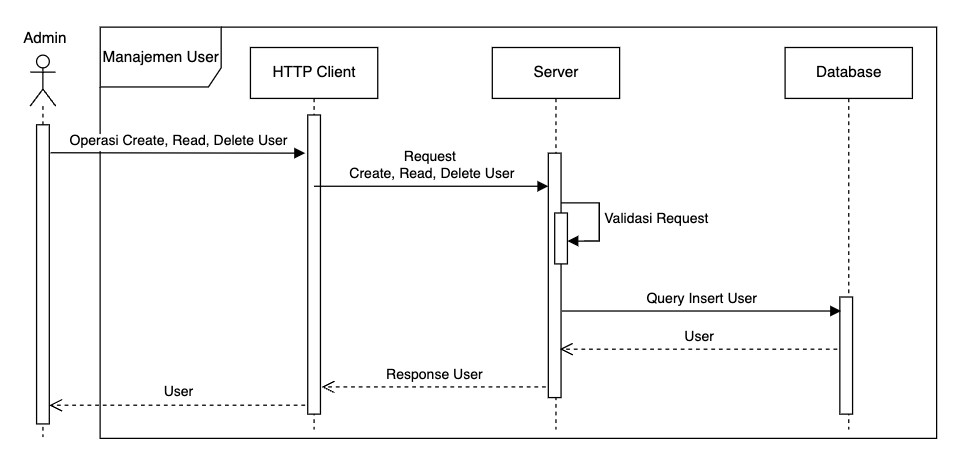
\includegraphics[width=1\textwidth]{resources/chapter-3/usecase/uc-04.jpg}
  \caption{\textit{Use Case} Manajemen \textit{User}}
  \label{fig:usecase-04}
\end{figure}

\subsubsection{Alur Login}

Pada \textit{use case} ini, \textit{user} dapat login ke dalam aplikasi dengan menginput kredensial berupa email dan password. Apabila data yang diberikan tidak valid, muncul modal untuk menandakan kesalahan yang dibuat. Apabila data benar, diberikan modal sukses lalu dilakukan \textit{redirect} ke halaman utama. Pada sisi server, terdapat beberapa validasi seperti apakah email terdapat di \textit{database} ataupun password match dengan hashed password yang ada di \textit{database}. Setelah itu, server memberikan response status ok dan memberikan \textit{user} akses ke halaman utama. Ilustrasi \textit{sequence diagram} dapat dilihat pada gambar \ref{fig:usecase-05}.

\begin{figure}[ht]
  \centering
  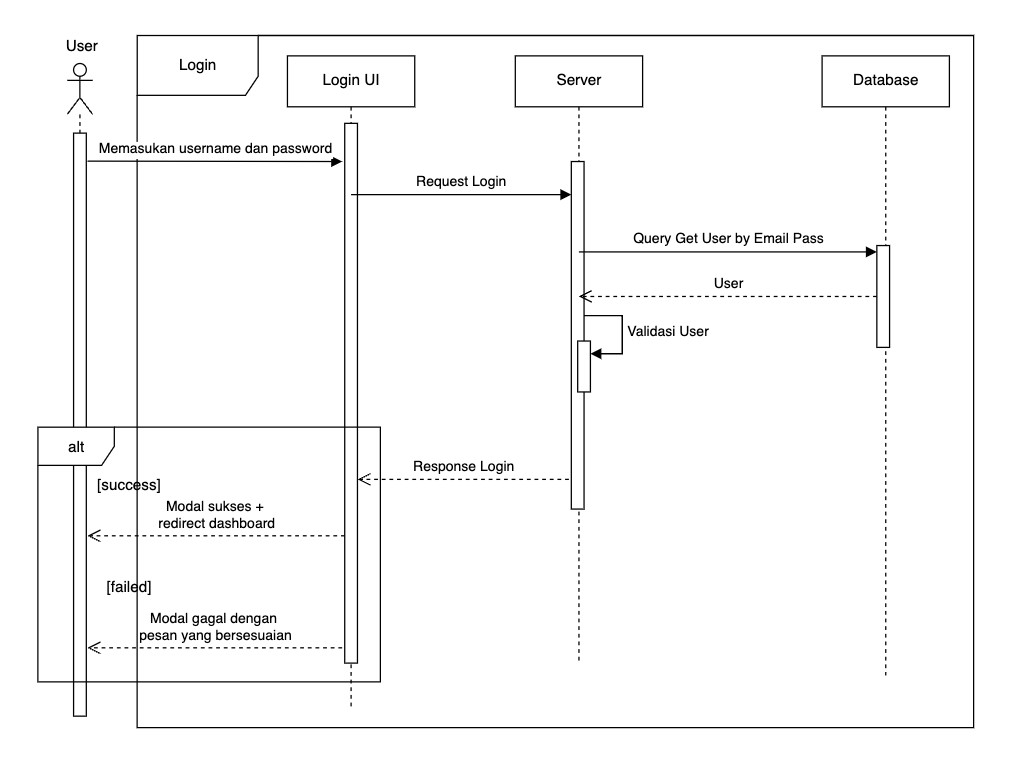
\includegraphics[width=0.8\textwidth]{resources/chapter-3/usecase/uc-05.jpg}
  \caption{\textit{Use Case} Alur Login}
  \label{fig:usecase-05}
\end{figure}

\pagebreak

\subsubsection{Alur Melihat detail \textit{company}}

Pada \textit{use case} ini, \textit{user} dapat melihat detail \textit{company} dengan cara mengunjungi halaman \textit{account}. Data diambil secara langsung melalui \textit{API Call} ke server, apabila terdapat error maka terdapat pesan error yang muncul. Apabila data berhasil di dapatkan, ditampilkan detail dari \textit{company} \textit{user}. Ilustrasi \textit{sequence diagram} dapat dilihat pada gambar \ref{fig:usecase-06}.

\begin{figure}[ht]
  \centering
  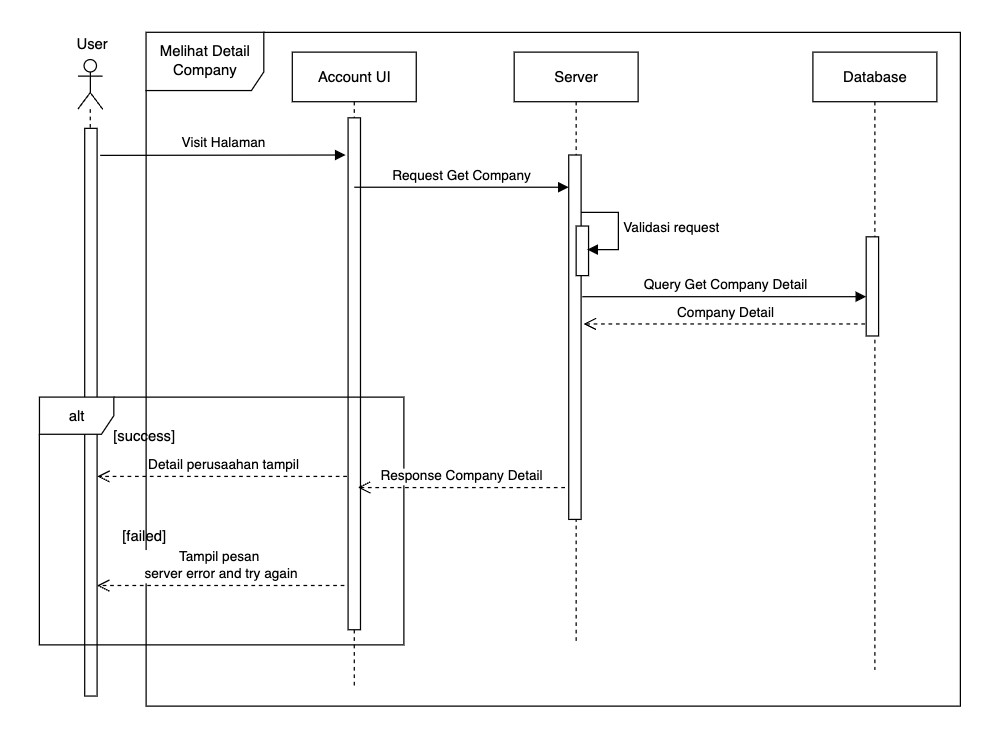
\includegraphics[width=0.8\textwidth]{resources/chapter-3/usecase/uc-06.jpg}
  \caption{\textit{Use Case} Melihat detail \textit{Company}}
  \label{fig:usecase-06}
\end{figure}

\subsubsection{Alur Melihat user lain di satu \textit{company}}

Pada \textit{use case} ini, \textit{user} dapat melihat detail seluruh user yang berada pada satu \textit{company} yang sama dengan cara mengunjungi halaman \textit{account}. Data diambil secara langsung melalui API Call ke server, apabila terdapat error maka terdapat pesan error yang muncul. Apabila data berhasil di dapatkan, ditampilkan daftar \textit{user} yang bersesuaian. Ilustrasi \textit{sequence diagram} dapat dilihat pada gambar \ref{fig:usecase-07}.


\begin{figure}[ht]
  \centering
  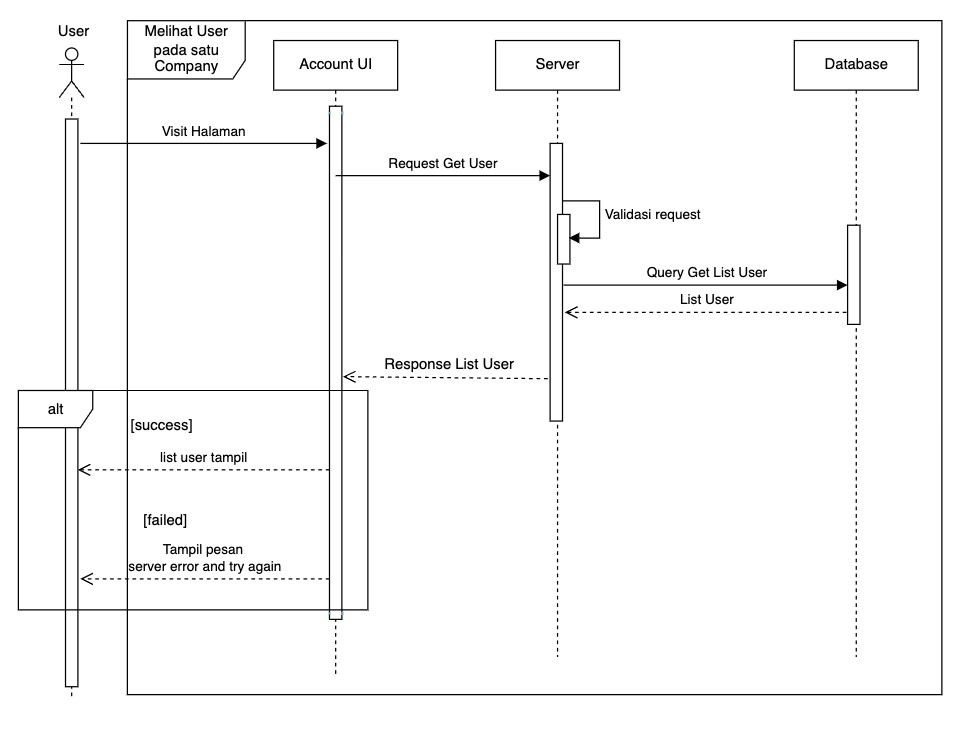
\includegraphics[width=1\textwidth]{resources/chapter-3/usecase/uc-07.jpg}
  \caption{\textit{Use Case} Melihat User Lain pada Satu \textit{Company}}
  \label{fig:usecase-07}
\end{figure}

\pagebreak

\subsubsection{Alur Manajemen \textit{Device}}

Pada \textit{use case} ini, \textit{user} dapat melakuakan manajemen \textit{device} dengan mengunjungi halaman \textit{devices}. Pada halaman ini \textit{user} dapat melakukan beberapa operasi yaitu mengambil daftar \textit{device} yang terdaftar, menambahkan \textit{device} baru, dan menghapus \textit{device}. Operasi pengambilan \textit{device} yang terdaftar dilakukan secara langsung ketika mengunjungi halaman. Operasi penghapusan ataupun penambahan \textit{device} dapat dilakukan oleh \textit{user} dengan cara menekan tombol yang ada pada laman. Ketika tombol ditekan terdapat validasi yang dilakukan pada halaman maupun pada server. Setelah melewati tahapan validasi, server melakukan update pada \textit{database}. Apabila terdapat error maka terdapat pesan error yang muncul. Apabila data berhasil di dapatkan, ditampilkan sebuah modal yang menandakan operasi berhasil untuk dilakukan. Ilustrasi \textit{sequence diagram} dapat dilihat pada gambar \ref{fig:usecase-08}.


\begin{figure}[ht]
  \centering
  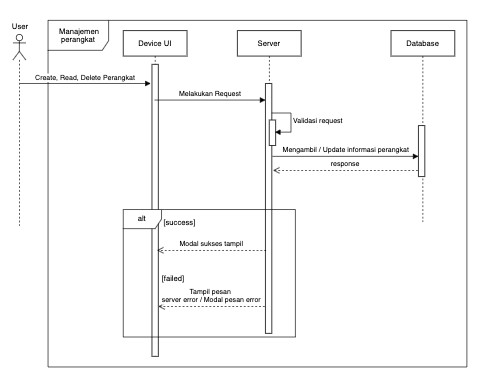
\includegraphics[width=1\textwidth]{resources/chapter-3/usecase/uc-08.jpg}
  \caption{\textit{Use Case} Manajemen \textit{Device}}
  \label{fig:usecase-08}
\end{figure}

\pagebreak

\subsubsection{Alur Manajemen \textit{Groups}}

Pada \textit{use case} ini, \textit{user} dapat melakuakan manajemen \textit{groups} dengan mengunjungi halaman \textit{groups}. Pada halaman ini \textit{user} dapat melakukan beberapa operasi yaitu mengambil daftar \textit{groups} yang terdaftar, menambahkan \textit{groups} baru, dan menghapus \textit{groups}. Operasi pengambilan \textit{groups} yang terdaftar dilakukan secara langsung ketika mengunjungi halaman. Operasi penghapusan ataupun penambahan \textit{groups} dapat dilakukan oleh \textit{user} dengan cara menekan tombol yang ada pada laman. Ketika tombol ditekan terdapat validasi yang dilakukan pada halaman maupun pada server. Setelah melewati tahapan validasi, server melakukan update pada \textit{database}. Apabila terdapat error maka terdapat pesan error yang muncul. Apabila data berhasil di dapatkan, ditampilkan sebuah modal yang menandakan operasi berhasil untuk dilakukan. Ilustrasi \textit{sequence diagram} dapat dilihat pada gambar \ref{fig:usecase-09}.


\begin{figure}[ht]
  \centering
  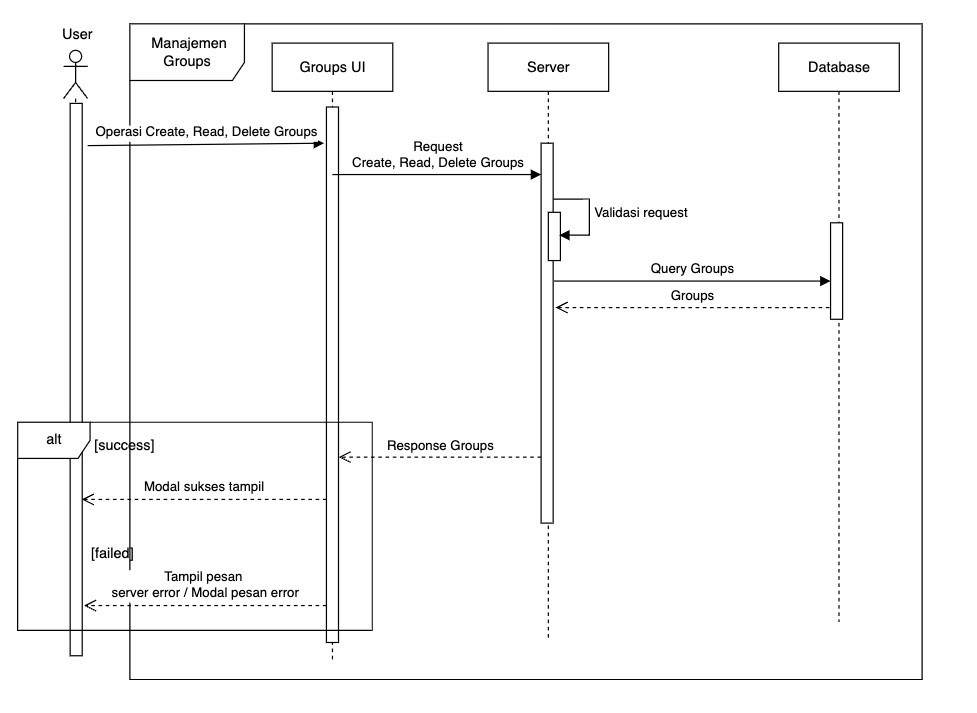
\includegraphics[width=1\textwidth]{resources/chapter-3/usecase/uc-09.jpg}
  \caption{\textit{Use Case} Manajemen \textit{Groups}}
  \label{fig:usecase-09}
\end{figure}

\pagebreak

\subsubsection{Alur Manajemen \textit{Deployment Images}}

Pada \textit{use case} ini, \textit{user} dapat melakuakan manajemen \textit{deployment images} dengan mengunjungi halaman \textit{deployments}. Pada halaman ini \textit{user} dapat melakukan beberapa operasi yaitu mengambil daftar \textit{deployment images}, menambahkan \textit{deployment images} baru, dan menghapus \textit{deployment images}. Operasi pengambilan \textit{deployment images} dilakukan secara langsung ketika membuka halaman. Operasi penghapusan ataupun penambahan \textit{deployment images} dapat dilakukan oleh \textit{user} dengan cara menekan tombol yang ada pada laman. Ketika tombol ditekan terdapat validasi yang dilakukan pada halaman maupun pada server. Setelah melewati tahapan validasi, server melakukan update pada \textit{database}. Apabila terdapat error maka terdapat pesan error yang muncul. Apabila data berhasil di dapatkan, ditampilkan sebuah modal yang menandakan operasi berhasil untuk dilakukan. Ilustrasi \textit{sequence diagram} dapat dilihat pada gambar \ref{fig:usecase-10}.

\begin{figure}[ht]
  \centering
  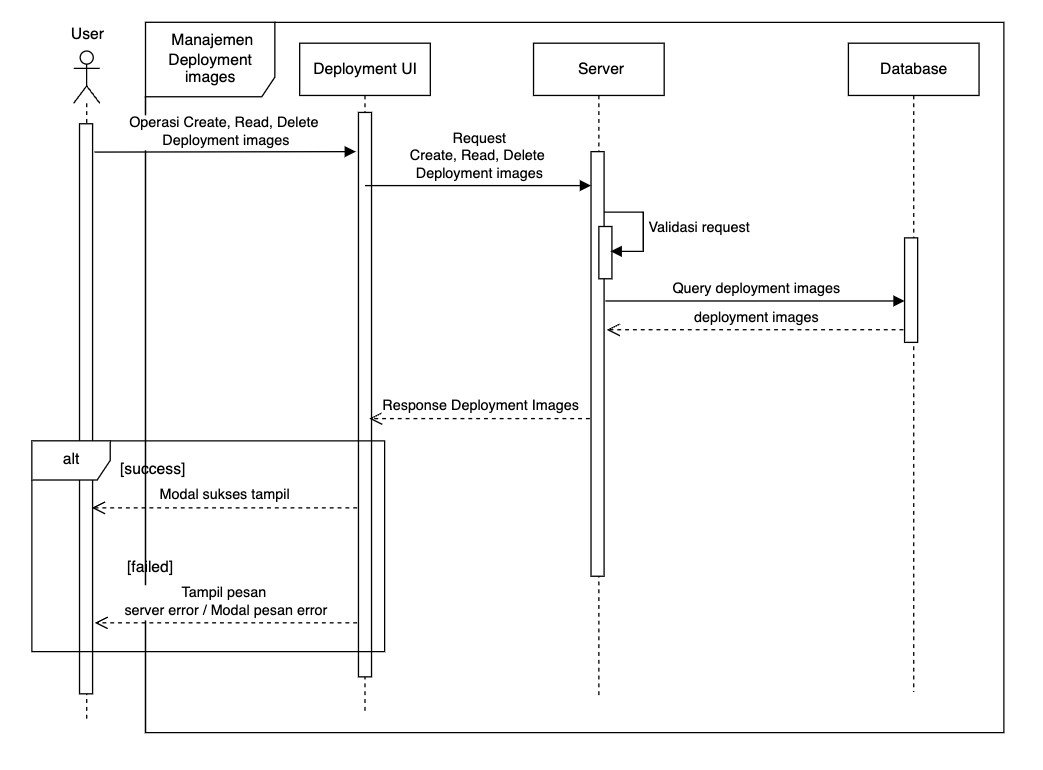
\includegraphics[width=1\textwidth]{resources/chapter-3/usecase/uc-10.jpg}
  \caption{\textit{Use Case} Manajemen \textit{Deployment Images}}
  \label{fig:usecase-10}
\end{figure}

\pagebreak

\subsubsection{Alur Manajemen \textit{Deployment Plan}}

Pada \textit{use case} ini, \textit{user} dapat melakuakan manajemen \textit{deployment plan} dengan mengunjungi halaman \textit{deployments}. Pada halaman ini \textit{user} dapat melakukan beberapa operasi yaitu mengambil daftar \textit{deployment plan} yang terdaftar, menambahkan \textit{deployment plan} baru, dan menghapus \textit{deployment plan}. Operasi pengambilan \textit{deployment plan} yang terdaftar dilakukan secara langsung ketika mengunjungi halaman. Operasi penghapusan ataupun penambahan \textit{deployment plan} dapat dilakukan oleh \textit{user} dengan cara menekan tombol yang ada pada laman. Ketika tombol ditekan terdapat validasi yang dilakukan pada halaman maupun pada server. Setelah melewati tahapan validasi, server melakukan update pada \textit{database}. Apabila terdapat error maka terdapat pesan error yang muncul. Apabila data berhasil di dapatkan, ditampilkan sebuah modal yang menandakan operasi berhasil untuk dilakukan. Ilustrasi \textit{sequence diagram} dapat dilihat pada gambar \ref{fig:usecase-11}.


\begin{figure}[ht]
  \centering
  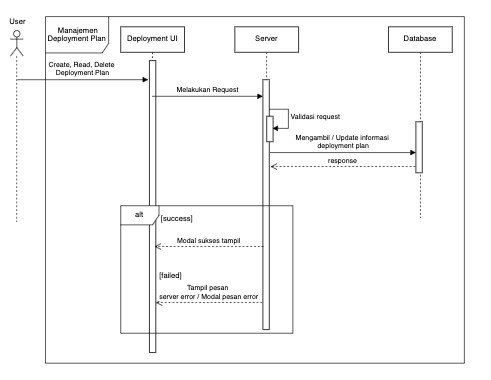
\includegraphics[width=1\textwidth]{resources/chapter-3/usecase/uc-11.jpg}
  \caption{\textit{Use Case} Manajemen \textit{Deployment Plan}}
  \label{fig:usecase-11}
\end{figure}

\pagebreak

\subsubsection{Alur \textit{remote deployment}}

Pada \textit{use case} ini, \textit{user} dapat melakukan \textit{remote deployment} dengan \textit{deployment plan} yang telah dibuat. Aksi ini dilakukan dengan cara mengunjungi halaman \textit{deployments} lalu menekan tombol deploy. Akan ada modal yang muncul memilih deployment yang dilakukan. Ketika user memilih deployment plan yang ingin di \textit{deploy}, terdapat validasi pada server sebelum melakukan deployment pada kubernetes. Setelah semua validasi berhasil dilakukan, kubernetes menginformasikan control plane pada cluster yang terhubung untuk memberikan perintah deploy kepada target. Balikan dari seluruh operasi ini adalah response berupa deployment berhasil dilakukan. Terdapat operasi \textit{asynchronus} pada \textit{background} untuk mengecek status deployment user. Ilustrasi \textit{sequence diagram} dapat dilihat pada gambar \ref{fig:usecase-12}.

\begin{figure}[ht]
  \centering
  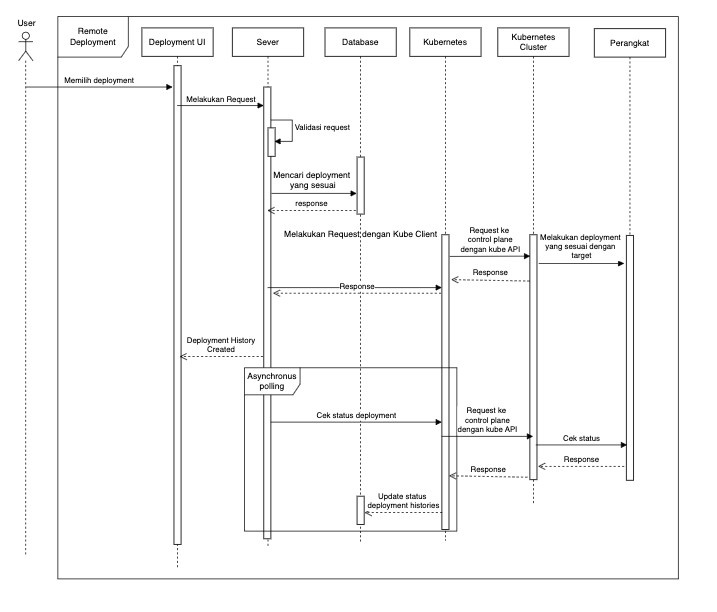
\includegraphics[width=1\textwidth]{resources/chapter-3/usecase/uc-12.jpg}
  \caption{\textit{Use Case} \textit{Remote Deployment}}
  \label{fig:usecase-12}
\end{figure}

\pagebreak

\subsubsection{Alur melihat riwayat \textit{deployment}}

Pada \textit{use case} ini, \textit{user} dapat melihat detail \textit{company} dengan cara mengunjungi halaman \textit{deployments}. Data diambil secara langsung melalui \textit{API Call} ke server, apabila terdapat error maka terdapat pesan error yang muncul. Apabila data berhasil di dapatkan, data menampilkan daftar \textit{deployment} apa saja yang telah dilakukan beserta statusnya. Ilustrasi \textit{sequence diagram} dapat dilihat pada gambar \ref{fig:usecase-13}.

\begin{figure}[ht]
  \centering
  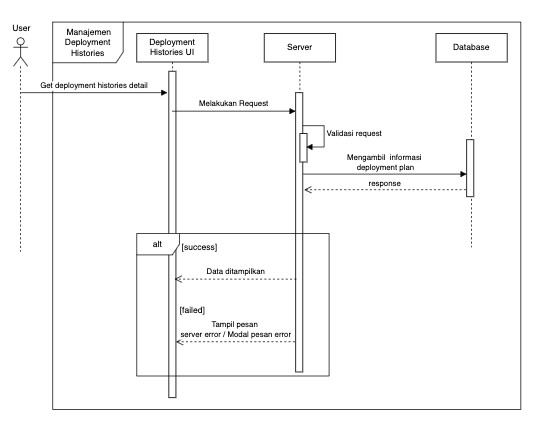
\includegraphics[width=1\textwidth]{resources/chapter-3/usecase/uc-13.jpg}
  \caption{\textit{Use Case} Melihat Riwayat \textit{Deployment}}
  \label{fig:usecase-13}
\end{figure}

\pagebreak